\documentclass[tikz, border=10pt]{standalone}
\usepackage{pgfplots}
\pgfplotsset{compat=1.18}

\begin{document}
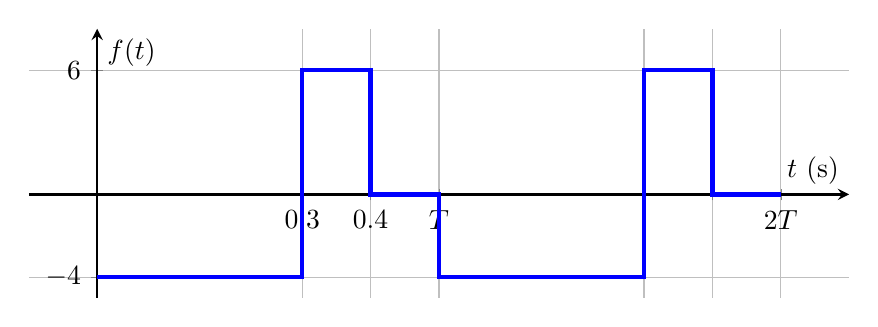
\begin{tikzpicture}
    \begin{axis}[
        width=12cm, height=5cm,
        axis lines=middle,
        xlabel={$t$ (s)}, ylabel={$f(t)$},
        ymin=-5, ymax=8,
        xmin=-0.1, xmax=1.1,
        xtick={0, 0.3, 0.4, 0.5, 0.8, 0.9, 1.0},
        xticklabels={0, 0.3, 0.4, $T$, , , $2T$},
        ytick={-4, 0, 6},
        grid=both,
        thick
    ]
        % Single continuous plot for both periods to ensure solid connected lines
        \addplot[blue, ultra thick] coordinates {
            (0, -4) 
            (0.3, -4)
            (0.3, 6)   % Vertical transition
            (0.4, 6)
            (0.4, 0)   % Vertical transition
            (0.5, 0)
            (0.5, -4)  % Vertical transition at T
            (0.8, -4)
            (0.8, 6)   % Vertical transition
            (0.9, 6)
            (0.9, 0)   % Vertical transition
            (1.0, 0)
        };
        
    \end{axis}
\end{tikzpicture}
\end{document}
